\usetikzlibrary{arrows}

\tikzstyle{int}=[draw, fill=blue!20, minimum size=2em]
\tikzstyle{init} = [pin edge={to-,thin,black}]

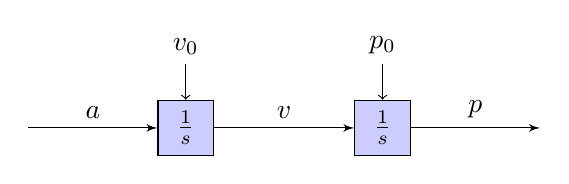
\begin{tikzpicture}[node distance=2.5cm,auto,>=latex']
    \node [int, pin={[init]above:$v_0$}] (a) {$\frac{1}{s}$};
    \node (b) [left of=a,node distance=2cm, coordinate] {a};
    \node [int, pin={[init]above:$p_0$}] (c) [right of=a] {$\frac{1}{s}$};
    \node [coordinate] (end) [right of=c, node distance=2cm]{};
    \path[->] (b) edge node {$a$} (a);
    \path[->] (a) edge node {$v$} (c);
    \draw[->] (c) edge node {$p$} (end) ;
\end{tikzpicture}